\section{Interacting scalar}
\label{section:interacting scalar}

We now study a scalar field with a $\lambda \varphi^4$ interaction term.
We write the Lagrangian in the form
\begin{equation*}
    \Ell = \Ell^{(0)} + \Ell^{(I)}, \quad 
    \Ell^{(0)} = 
    \frac{1}{2} \partial_\mu \varphi \partial^\mu \varphi - m^2 \varphi^2 , \quad
    \Ell^{(I)} = - \frac{\lambda}{4!} \varphi^4
\end{equation*}
$\Ell^{(I)}$ is called the interaction term, and makes it impossible to exactly solve for the partition function.
Instead, we turn to perturbation theory.
The canonical partition function in this theory is
\begin{equation}
    Z = \Tr{e^{- \beta \hat H}}
    = \int_S \D \varphi \, \exp{
        - \int_\Omega \dd X \left(\Ell_E^{(0)} + \Ell_E^{(I)}\right)
    }
    = \int_S \D \varphi \, e^{-S_0} e^{-S_I}.
\end{equation}
Here, $S_0$ and $S_I$ denote the Euclidean action due to the free and interacting Lagrangian, respectively.
The domain of integration $S$ is again periodic field configurations $\varphi(\beta, \vec x) = \varphi(0, \vec x)$.
We may write the free energy as
\begin{equation*}
    - \beta F = \ln
    \left[
        \int_S \D \varphi \, e^{-S_0} \sum_n \frac{1}{n!} {(-S_I)}^n
    \right]
    = \ln[Z_0] 
    + \ln
    \left[
        Z_I
    \right],
\end{equation*}
where $Z_0$ is the partition function of the free theory.
The correction to the partition function is thus given by
\begin{equation}
    Z_I = \sum_{n=0}^\infty \frac{(-1)^n}{n!} \ex{{S_I}^n}_0,
\end{equation}
where
\begin{equation}
    \ex{A}_0 = \frac{
        \int_S \D \varphi \, A \, e^{-S_0} }
    {\int_S \D \varphi \, e^{-S_0}}.
\end{equation}

To evaluate expectation values of the form $\ex{\varphi(X_1) ... }_0$, we introduce the partition function with a source term
\begin{align}
    Z[J] = \int_S \D \varphi \, \exp{
        - \frac{1}{2} \int_\Omega \dd X \, \varphi (-\partial_E^2 + m^2) \varphi
        + \int_\Omega \dd X \, J \varphi
    }.
\end{align}

Thermal propagators are the generalization of the time-ordered two-point functions $\ex{T\{\varphi(x) \varphi(y) \}}$ of the vacuum formalism.
For some differential operator $D^{-1}$, the thermal propagator is defined as
\begin{equation}
    D^{-1} D(X, Y) = \beta \delta(X - Y).
\end{equation}
The Fourier transformed propagator is, assuming $D(X, Y) = D(X-Y, 0)$,
\begin{align}
    \nonumber
    \tilde D(K, K') 
    & = \frac{1}{V \beta^3} \int_{\Omega} \dd X \dd Y \, 
    D(X, Y) \exp(- i [X\cdot K + Y\cdot K']) \\ \nonumber
    & = \frac{1}{V \beta^3} \int_{\Omega} \dd X' \dd Y' \, D(X', 0) 
    \exp(- i [X'\cdot \frac{1}{2} (K - K') + Y\cdot (K + K')]) \\
    & = \frac{1}{V \beta^2} \tilde D(K) \delta(K + K'),
\end{align}
where
\begin{equation}
    \tilde D(K) = \int \dd X e^{iK\cdot X} D(X, 0).
\end{equation}
We write the thermal propagator of the free field as $D_0(X, Y)$.
With this, we may complete the square,
\begin{align}
    Z[J] = Z[0]\exp{\frac{1}{2} \int_{\Omega} \dd X \dd Y J(X) D_0(X, Y) J(Y)}
    = Z[0] \exp(W[J])
\end{align}
We can now write
\begin{equation}
    \ex{\varphi(X)\varphi(Y)}_0 
    = \frac{1}{Z[0]}
    \frac{\delta}{\delta J(X)} \frac{\delta}{\delta J(Y)} 
    Z[J] \Big|_{J=0} 
    = D_0(X, Y),
\end{equation}
This generalizes to higher order expectation values,
\begin{equation}
    \ex{\varphi(X_i) \dots \varphi(X_n)}_0
    = \left(\prod_{i=1}^n \frac{\delta}{\delta J(X_i)}\right) 
    Z[J] \Big|_{J=0},
\end{equation}

Using Wick's theorem, as described in \autoref{section:path integral}, the expectation values we are evaluating can be written
\begin{align*}
    \ex{{S_I}^m} & 
    = \left(- \frac{\lambda }{4!}\right)^m 
    \int_{\Omega} \dd X_1 \dots \dd X_m
    \ex{\varphi^4(X_1) \dots \varphi^4(X_m)} \\ 
    & \quad
    = \left(- \frac{\lambda }{4!}\right)^m 
    \int_{\Omega} \dd X_1 \dots \dd X_m \sum_{\{a, b\}}
    \ex{\varphi(X_{a(1)}) \varphi(X_{b(1)})} 
    \dots
    \ex{\varphi(X_{a(2m)}) \varphi(X_{b(2m)})}
\end{align*}
where $X_i$ for $i>m$ is defined as $X_j$, where $j = i \mod m$.
This means that $X_{m + i} = X_i$.
The functions $a,\,b$ represents a possible pairing, as described in \autoref{section:path integral}.
Inserting the Fourier expansions of the field gives
\begin{align*}
    & \ex{{S_I}^m} \\ 
    &\quad 
    = \left(-\frac{\lambda }{4!}\right)^m 
    \int_{\Omega} \dd X_1 \dots \dd X_m
    (V \beta)^2 \int_{\tilde \Omega} \dd K_1 ... \dd K_{2m} \sum_{\{a, b\}} \\
    & \quad \quad \quad \quad\quad \quad \quad
    \ex{\varphi(K_{a(1)}) \varphi(K_{b(1)})} 
    \dots
    \ex{\varphi(K_{a(2m)}) \varphi(K_{b(2m)})}     
    \exp(i {\sum}_{i=1}^{m} X_i \cdot K_i)\\ 
    & \quad  
    = \left(-\frac{\lambda }{4!}\right)^m 
    \frac{(V \beta)^{2m} \beta^m}{(V \beta^2)^{2m}}
    \int_{\tilde \Omega} \dd K_1 ... \dd K_{2m} \sum_{\{a, b\}} \\
    & \quad \quad \quad \quad \quad \quad \quad \quad \quad
    \tilde D(K_{a(1)}) \delta(K_{a(1)} + K_{b(1)}) \dots 
    \tilde D(K_{a(2m)}) \delta(K_{a(2m)} + K_{b(2m)})
    \prod_{i=1}^m \delta\left(X_i \cdot {\sum}_{j=0}^3 K_{i + jm}\right) \\
    & \quad 
    = \left(-\frac{\lambda \beta}{4!}\right)^m 
    \prod_{i=1}^{2m} \int_{\tilde \Omega} 
    \left( \dd K_i \frac{1}{\beta} \tilde D(K_i)  \right) 
    \prod_{i=1}^m \delta\left(X_i \cdot {\sum}_{j=0}^3 K_{i + jm}\right)
    \sum_{\{a, b\}} 
    \prod_{n=1}^{2m}\delta(K_{a(k)} + K_{b(k)})
\end{align*}
Here we have used that $V \beta^2 \tilde D_0(K, P) = \tilde D_0(K) \delta(P + K)$, where $\tilde D_0(K)$ is the thermal propagator for the free field.
In this case, it is
\begin{equation}
    \tilde D_0(K) = \tilde D_0(\omega_n, \vec k) = \frac{1}{\omega_k^2 + \omega_n^2}.
\end{equation}
This expectation value can be represented graphically using Feynman diagrams.
The thermal $\lambda \varphi^2$-theory gets the prescription

\begin{align}
    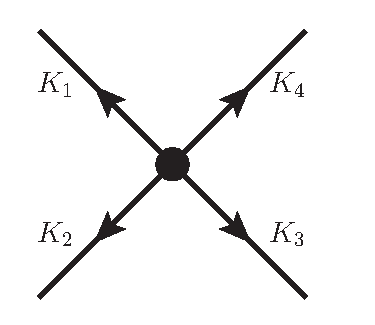
\includegraphics[width=0.15\textwidth, valign=c]{figurer/feynman-diagram/phi-4_vertex.eps}
    & = -\lambda \beta
    \delta \left({\sum}_i K_i \right), \\ \nonumber \\
    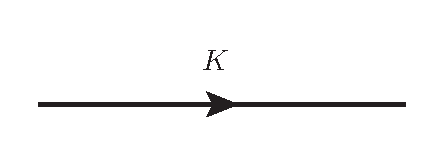
\includegraphics[width=0.2\textwidth, valign=c]{figurer/feynman-diagram/phi-4_propagator.eps}
    & = \frac{1}{\beta} D_0(K).
\end{align}
Lastly, one has to integrate over all internal momenta, and divide by a symmetry factor of the diagram $s$, which is described in detail in~\cite{Peskin:IntroQFT}.

Calculating $\ex{{S_I}^n}_0$ boils down to the sum of all possible Feynman diagrams with $n$ vertices.
The first example is 
\begin{align}
    \ex{S_I} = 
    \frac{1}{8} 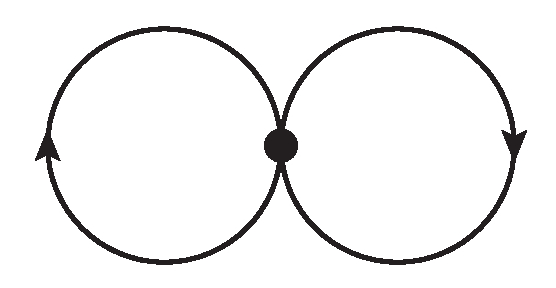
\includegraphics[width=0.15\textwidth, valign=c]{figurer/feynman-diagram/phi-4_loop_notext.eps}.
\end{align}

In \autoref{section:path integral}, we saw that the sum of all vacuum diagrams is the exponential of the sum of all \emph{connected} diagrams, so the free energy of the interacting theory is given by
\begin{equation}
    - \beta F = \ln(Z_0) + \Sigma(\mathrm{all\,\, connected\,\, diagrams}).
\end{equation}
